\section{From packing density to the control problem}\label{sec:setting}

The useful normalization fixes the area of a densest lattice cell. For a worst disk, the contact
points of these lattice packings then describe a moving hexagon of fixed area. This section
explains how the motion becomes a control problem and why its cost gives the required packing
bound. The coordinate formulas and regularity conditions are in \cref{app:setup}.

\subsection{Packing densities}\label{sec:set-packings}

A \emph{convex disk} is a compact convex set $K\subset\R^2$ with nonempty interior. It is
\emph{centrally symmetric} if it has a centre $c$, so that $2c-x\in K$ for every $x\in K$. A
\emph{congruent copy} of $K$ is its image under a Euclidean isometry, which may reverse the
orientation. A \emph{packing} is a family of convex disks with pairwise disjoint interiors. Let
$B_r$ be the closed disk of radius $r$ about the origin.

\begin{definition}[Greatest packing density]\label{def:packing-density}
The \emph{density} of a packing $\mathcal P$ exists if the limit
\[
  \delta(\mathcal P)=\lim_{r\to\infty}\frac{1}{\area(B_r)}\sum_{K'\in\mathcal P}\area(K'\cap B_r)
\]
exists and is finite, that is, if the upper and lower limits are equal and finite. The
\emph{greatest packing density} $\delta(K)$ of a convex disk $K$ is the supremum of
$\delta(\mathcal P)$ over the packings $\mathcal P$ by congruent copies of $K$ whose density
exists \cite[Def.~2.1.1]{HalesVajjha2024}.
\end{definition}

A \emph{lattice} is a discrete subgroup $L=\Z b_0+\Z b_1$ of $\R^2$ with $b_0,b_1$ linearly
independent; its determinant is $\det L=\abs{\det(b_0,b_1)}$. If the translates $K+v$, $v\in L$,
form a packing, its density exists and equals $\area(K)/\det L$. The \emph{greatest lattice packing
density} $\delta_L(K)$ is the supremum of these values.

\begin{theorem}[Fejes T\'oth~\cite{FejesToth1950}, Rogers~\cite{Rogers1951}]\label{thm:fejes-toth}
For every centrally symmetric convex disk $K$, $\delta(K)=\delta_L(K)$.
\end{theorem}

So for centrally symmetric disks the problem is a problem about lattices. A linear map carries
lattice packings to lattice packings and multiplies areas and determinants by the same factor, so
$\delta(K)$ is invariant under invertible affine maps (\cref{prop:converse}). The \emph{minimax
density} $\delta_{\min}$ is the infimum of $\delta(K)$ over all centrally symmetric convex disks,
and a \emph{worst disk} is a centrally symmetric convex disk, centred at the origin, with
$\delta(K)=\delta_{\min}$. Worst disks exist, by Blaschke's selection theorem and the continuity of
$\delta_L$ in the Hausdorff metric (Reinhardt~\cite{Reinhardt1934}, Mahler~\cite{Mahler1947b};
\cite[\S2.2]{HalesVajjha2024}). In this language the conjecture says that $\delta_{\min}=\doct$ and
that the worst disks are the linear images of the smoothed octagon.

\subsection{A moving hexagon on the boundary}\label{sec:setting-hexagon}

The lattice description gives more than a formula for density. A densest lattice packing can be
described by six contact points on the boundary of the disk. They occur in opposite pairs and form an
\emph{affinely regular hexagon}, the image of a regular hexagon under an invertible affine map.
For a worst disk, Reinhardt's theory supplies a continuous family of such hexagons whose vertices
sweep out the entire boundary. The family allows us to study the disk through the motion of six
points.

Normalize one contact hexagon to the regular hexagon with vertices
\[
  s_j=(\cos(j\pi/3),\sin(j\pi/3)),\qquad j=0,\ldots,5.
\]
The associated packing lattice has cell area $\sqrt{12}$. Write $\sigma_j(t)$ for the six moving
contact points, with $t$ a parameter along the motion. Their hexagon has constant area. There is
therefore a unique area-preserving linear map $g(t)$ carrying every $s_j$ to $\sigma_j(t)$.
We call $g(t)$ the \emph{frame}. In matrix notation it belongs to
$\SLtwo$, the group of real $2\times2$ matrices with determinant one.

A suitable choice of the parameter gives a number $T>0$ such that
$\sigma_j(T)=s_{j+1}$, with the index read modulo six. Thus, during $[0,T]$, each contact point
traces one part of the boundary. The six parts together trace the whole boundary. This is the
period used in the control problem; the individual points return to their initial positions
after six such periods. The exact conditions on the contact curves are expressed by a
\emph{balanced pair}, defined in \cref{def:balanced}.

\subsection{The state, the control and the cost}\label{sec:setting-control}

The velocity of the frame is recorded by the matrix
\[
  X(t)=g(t)^{-1}g'(t),\qquad\text{so that}\qquad g'(t)=g(t)X(t).
\]
This is the \emph{state}. Since $g$ preserves area, $X$ has trace zero. We choose the time
parameter so that $\det X=1$. The geometric restrictions on the contact curves require $X$ to
lie in a specified open set of such matrices, called the \emph{star states}
(\cref{sec:set-control}).

Convexity requires nonnegative curvature of the contact curves. Hales expresses the allowed
curvatures by a \emph{control} $u(t)=(u_0(t),u_1(t),u_2(t))$, where
\[
  u_i(t)\ge0,\qquad u_0(t)+u_1(t)+u_2(t)=1.
\]
The possible controls form a triangle, denoted $\UT$. Its three vertices are the coordinate
vectors $\ee_0=(1,0,0)$, $\ee_1=(0,1,0)$ and $\ee_2=(0,0,1)$. A control determines the evolution
of $X$ through the second state equation in \cref{def:control-problem}. At a vertex control,
three contact curves trace straight segments and the other three trace hyperbolic arcs. This
explains why sequences of vertex controls produce smoothed polygons.

Let $I$ be the identity matrix and $R$ the rotation through $\pi/3$. The closing conditions are
\[
  g(0)=I,\qquad g(T)=R,\qquad X(T)=R^{-1}X(0)R.
\]
The frame and its velocity then fit together when the contact points are relabeled. A solution
of the state equations satisfying these conditions is an \emph{admissible trajectory}, written
$(T,u,g,X)$. The terminal time $T$ is allowed to vary, and the control is only required to be
measurable. These conditions are stated precisely in \cref{def:control-problem}.

The \emph{cost} $\cost(T,X)$ is the area integral of the six contact curves
(\cref{eq:cost}). For a balanced disk $K$ it satisfies
\[
  \cost(T,X)=\area(K)=\sqrt{12}\,\delta(K).
\]
Thus minimizing the cost is the normalized version of finding the worst packing density.

\subsection{The octagon as a reference motion}\label{sec:setting-reference}

Reinhardt's smoothed octagon $\Koct$ has eight straight boundary segments joined tangentially by
eight hyperbolic arcs. Its exact construction is given in \cref{def:smoothed-octagon}.
Hales represents an affine image of this disk by four pieces of constant control with labels
$2,0,1,2$. The pieces have equal durations. The resulting trajectory is admissible and has cost
$\Aoct=\sqrt{12}\,\doct<\pi$ (\cref{prop:octagon-trajectory}).

We denote the disk in this normalization by $\KH$. The disks $\KH$ and $\Koct$ differ by an
explicit invertible linear map (\cref{prop:reinhardt-construction}), so they have the same packing
density. In particular, the octagon supplies a reference cost against which every global minimizer
can be compared.

\begin{figure}[htbp]
  \centering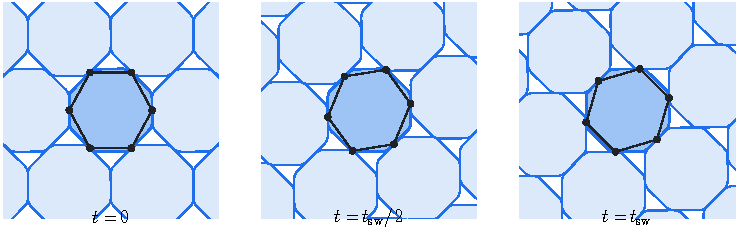
\includegraphics[width=\textwidth]{figures/fig-packing.pdf}
  \caption{Three densest lattice packings of the smoothed octagon. The dark copy touches six
  neighbours in each packing. The contact points move along its boundary as the packing lattice
  varies, while the density remains $\doct$.}
  \label{fig:packing}
\end{figure}

\begin{figure}[htbp]
  \centering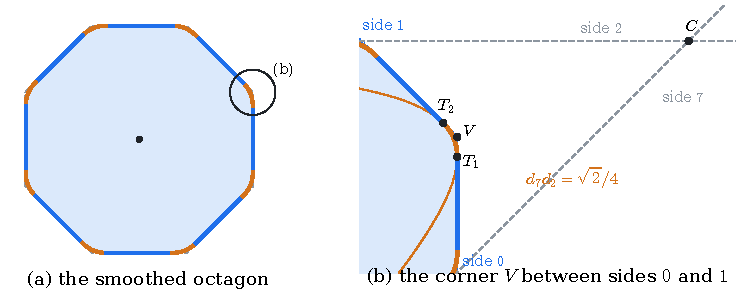
\includegraphics[width=\textwidth]{figures/fig-octagon.pdf}
  \caption{(a) The smoothed octagon: straight boundary segments (blue) and hyperbolic arcs
  (orange) inside the regular octagon (dashed). (b) One corner is replaced by the arc from $T_1$
  to $T_2$. The hyperbola is tangent to the two sides at these points and asymptotic to the
  neighbouring side lines, which meet at $C$. The coordinates are given in \cref{sec:set-octagon}.}
  \label{fig:octagon}
\end{figure}

\subsection{Why the geometric and control minima agree}\label{sec:setting-equivalence}

A \emph{global minimizer} is an admissible trajectory whose cost is no greater than that of any
other admissible trajectory, including trajectories with a different terminal time
(\cref{def:global-minimizer}). To use a cost bound for the packing problem, we must know that a
worst disk gives such a minimizer. Two geometric comparisons establish this.

First, a worst disk can be normalized and parametrized by an admissible trajectory whose cost is
$\sqrt{12}$ times its density (\cref{prop:realization}). Second, every admissible trajectory of
cost below $\pi$ traces a balanced disk with the same area (\cref{prop:reverse-comparison}). In
this second comparison the cost bound ensures that the contact curves go around the boundary
once, so that they describe a convex disk.

The octagon costs less than $\pi$. Any trajectory that could improve on the realization of a
worst disk would therefore also have cost below $\pi$, and would produce a disk with a smaller
packing density. This contradicts the choice of a worst disk. Its realization is consequently a
global minimizer. The same comparisons prove the equivalence between the lower bound for all
packing densities and the lower bound for all admissible costs (\cref{thm:equivalence}).

There is also a geometric restriction on the states that need to be considered. Hales and Vajjha
show that the state of every global minimizer lies in a fixed compact set, denoted $\hstarstar$
(\cref{thm:compact-domain}). In particular it stays away from the boundary of the allowed state
domain. This restriction will enter the last mixed case. The next section reduces the control
of a minimizer to a finite sequence of vertex choices.
